
\chapter{Modeling} \label{ch:modeling}

In order to choose the methods best suited for solving the problems presented in \chapref{ch:intro} a representative model of the system is needed. This model must thus contain all the physical phenomena which is needed to facilitate methods for solving the presented problems. These phenomena are contact surface pressure responses from the object's texture and topology to the manipulator and frictions between the object and manipulator. Modeling these is done by applying contact and friction models respectively. \medskip

To illustrate a single point contact model between the \gls{ee}'s finger and the object, a normal force $\mathbf{f}_N$ at contact point $\mathbf{c}_1$ can be seen in \figref{fig:contact-single-point}. Once a greater force is applied by the \gls{ee}'s finger the point contact expands to a contact surface which due to the finger's surface being compliant and said finger's convex shape a pressure distribution $p(r)$ is created. The pressure distribution is here a function of the contact surface radius $r$ assuming a non-conforming contact case. This can be seen illustrated in \figref{fig:contact-surface}

\begin{center}
    \renewcommand{\arraystretch}{1.2}
    \begin{minipage}{.48\linewidth}
        \vspace{0pt}
        \centering
        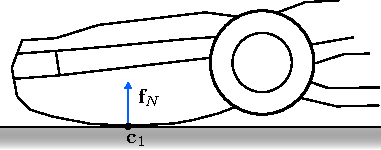
\includegraphics[width=.95\textwidth]{chapters/modeling/fig/contact-single-point.pdf}
    \end{minipage}%
    \hfill%
    \begin{minipage}{.48\linewidth}
        \vspace{0pt}
        \centering
        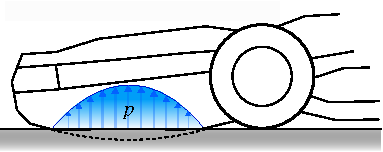
\includegraphics[width=.95\textwidth]{chapters/modeling/fig/contact-surface.pdf}
    \end{minipage}%
    %    
    \vspace{15pt}
    %
    \begin{minipage}[t]{.48\linewidth}
        \vspace{0pt}
        \captionsetup{type=figure}
        \captionof{figure}{Single point contact model between compliant manipulator surface and object surface.}
        \label{fig:contact-single-point}
    \end{minipage}%
    \hfill%
    \begin{minipage}[t]{.48\linewidth}
        \vspace{0pt}
        \captionsetup{type=figure}
        \captionof{figure}{Contact model of the pressure distribution $p(r)$ caused by the increased force applied from the \gls{ee}'s finger to the object.}
        \label{fig:contact-surface}
    \end{minipage}%
\end{center}

An illustration of a point contact friction model can be seen in figure \figref{fig:friction-single-point}, where $\mathbf{c}_1$ is the point of contact, $\mathbf{f}_N$ is the normal force acting on the \gls{ee}'s finger in $\mathbf{c}_1$, $\mathbf{f}_f$ is the friction force reacting to the external force acting on the object $\mathbf{f_{\text{ext}}}$. The friction force will here be proportional to the normal force applied by the \gls{ee}'s finger.\medskip

When the \gls{ee} applies a greater force on the object the normal force will likewise increase and thus the friction force will increase. This model considers the finger to be compliant and thus a soft finger friction model can be utilized. The soft finger friction model can be seen in \figref{fig:friction-surface}

\begin{center}
    \renewcommand{\arraystretch}{1.2}
    \begin{minipage}{.48\linewidth}
        \vspace{0pt}
        \centering
        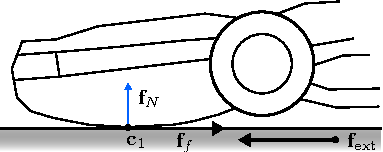
\includegraphics[width=.95\textwidth]{chapters/modeling/fig/friction-single-point.pdf}
    \end{minipage}%
    \hfill%
    \begin{minipage}{.48\linewidth}
        \vspace{0pt}
        \centering
        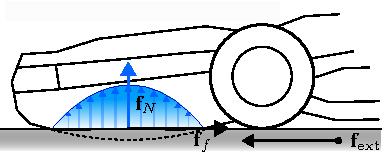
\includegraphics[width=.95\textwidth]{chapters/modeling/fig/friction-surface.pdf}
    \end{minipage}%
    %    
    \vspace{15pt}
    %
    \begin{minipage}[t]{.48\linewidth}
        \vspace{0pt}
        \captionsetup{type=figure}
        \captionof{figure}{Single point contact model between compliant manipulator surface and object surface.}
        \label{fig:friction-single-point}
    \end{minipage}%
    \hfill%
    \begin{minipage}[t]{.48\linewidth}
        \vspace{0pt}
        \captionsetup{type=figure}
        \captionof{figure}{Friction model of the pressure distribution $p(r)$ caused by the increased force applied from the \gls{ee}'s finger to the object.}
        \label{fig:friction-surface}
    \end{minipage}%
\end{center}

During in-hand manipulation the presence of external forces is a common problem and often comes in the form of gravity acting on the object, which can cause the problem to slip. By combining the contact and friction models as described above grasps and in-hand manipulations can be performed by compensating for the gravitational pull with applied force. This can be seen illustrated in \figref{fig:contact-friction-model}. \medskip

By describing the kinematic tree of the \gls{ee}, the 

\begin{center}
    \renewcommand{\arraystretch}{1.2}
    \begin{minipage}{.48\linewidth}
        \vspace{0pt}
        \centering
        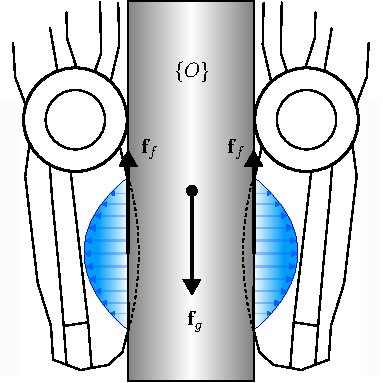
\includegraphics[width=.95\textwidth]{chapters/modeling/fig/contact-friction-model.pdf}
    \end{minipage}%
    \hfill%
    \begin{minipage}{.48\linewidth}
        \vspace{0pt}
        \centering
        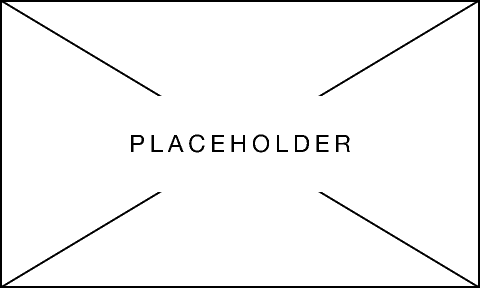
\includegraphics[width=.95\textwidth]{img/placeholder.png}
    \end{minipage}%
    %    
    \vspace{15pt}
    %
    \begin{minipage}[t]{.48\linewidth}
        \vspace{0pt}
        \captionsetup{type=figure}
        \captionof{figure}{The friction forces $\mathbf{f}_f$ and contact model keeps the object $\{O\}$ from slipping between the \gls{ee}'s fingers when the gravitational pull $\mathbf{f}_g$ is acting on it.}
        \label{fig:contact-friction-model}
    \end{minipage}%
    \hfill%
    \begin{minipage}[t]{.48\linewidth}
        \vspace{0pt}
        \captionsetup{type=figure}
        \captionof{figure}{The model of the world representation for this project.}
        \label{fig:full-system-model}
    \end{minipage}%
\end{center}

To determine which methods best describe the models presented above for this project, the \gls{sota} will be presented in \chapref{ch:state-of-the-art}.


